\scanpage{66}
% archive sheet number: 65
% @ L1–5, cancelled continuation
\deleted{\deleted{\unsure{sont}} envisageables il y a une application canonique de la surface vrillée dans $X$ ! \deleted{Si on recolle par} \inserted{Non, c'est vrai pourvu} \deleted{\unsure{donc|dès}} que, pour $\alpha$ choisi, on choisisse l'identification}

% @ L6–12
Si on veut une application naturelle de la surface vrillée dans $X$, qui sur $\Delta_D,\Delta_{D'}$ se réduise au plongement canonique, il faut \inserted{(semble-t-il)} que $b$ et $\alpha$ se réalisent par le $=$ segment plongé dans $X$, ce qui \inserted{semble} imposer $\alpha=a'$ ! Mais si on convient de remplacer $\Delta_D$ par un disque un peu plus petit $\Delta_D^*$ \inserted{dont le bord} passant par $s$ (cf pointillé ci-contre), et déplace en conséquence $b$ en $b^*$, et faire le vrillement le long de $b^*$ plutôt que $b$, \deleted{donc} et pareil pour le disque $\Delta_{D'}$,

% @ L, inset beside passant par s
\figure{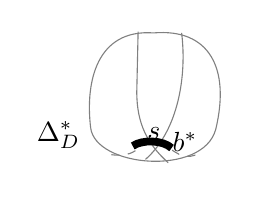
\begin{tikzpicture}[x=.85cm,y=.85cm]
\draw[gray] (0,.98) .. controls (-.85,1.04) and (-1.02,.25) .. (-.94,-.43) .. controls (-.88,-1.03) and (.74,-1.17) .. (.93,-.46) .. controls (1.15,.46) and (.83,1.05) .. (0,.98);
\draw[gray] (-.23,1)--(-.25,.1) .. controls (-.25,-.38) and (-.09,-.68) .. (.22,-.96);
\draw[gray] (.42,.98) .. controls (.5,.34) and (.37,-.48) .. (-.12,-.91);
\draw[thin,dashed,gray] (-.63,-.84) .. controls (-.23,-.89) and (-.22,-.66) .. (0,-.64) .. controls (.24,-.65) and (.36,-.97) .. (.66,-.83);
\draw[line width=2.8pt] (-.31,-.71) .. controls (-.17,-.61) and (.14,-.62) .. (.27,-.74);
\node at (.005,-.52) {$s$};\node at (.47,-.65) {$b^*$};\node at (-1.42,-.55) {$\Delta_D^*$};
\end{tikzpicture}}

% @ L, final five lines
(de façon à faire \unsure{coïncider|coincider} les images de $a$ et $a'$ dans $X$), on voit qu'on arrivera à \deleted{faire appliquer} \inserted{trouver} une application de la surface vrillée dans $X$, même en choisissant $\alpha=a$.

% @ L last line to R1–3
Le choix le plus naturel quand même (\deleted{dans} pt de vue application dans $X$) semblerait $\alpha=a'$. Donc sur le terrain cela donne -- \uline{continuation}

% @ R, below continuation
\figure{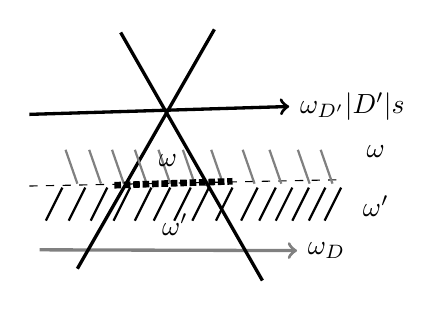
\begin{tikzpicture}[x=1cm,y=1cm]
\draw[->,very thick] (-1.75,.76)--(1.55,.86) node[right] {$\unsure{\omega_{D'}|D'|s}$};
\draw[->,very thick,gray] (-1.62,-.96)--(1.65,-.97) node[right,black] {$\omega_D$};
\draw[very thick] (-1.14,-1.2)--(.60,1.84) (-.59,1.8)--(1.21,-1.35);
\draw[dashed,thin] (-1.75,-.15)--(2.2,-.07);
\foreach \x in {-1.14,-.84,-.55,-.26,.04,.35,.71,1.11,1.45,1.81,2.1}{\draw[thick,gray] (\x,-.12)--++(-.15,.43);}
\foreach \x in {-1.33,-1.04,-.76,-.47,-.2,.04,.3,.53,.83,1.15,1.38,1.59,1.8,2.01,2.21}{\draw[thick] (\x,-.17)--++(-.21,-.42);}
\draw[line width=2.4pt,densely dotted] (-.67,-.14)--(.83,-.09);
\node at (.01,.18) {$\omega$};\node at (.10,-.64) {$\omega'$};
\node at (2.65,.29) {$\circlearrowleft\omega$};\node at (2.65,-.4) {$\circlearrowleft\omega'$};
\end{tikzpicture}}
% @ R4–8
d'une rive par la suivante -- l'application $\mathscr X\to X$ est une \uline{immersion}.

% @ R9–end
Dans cette optique \inserted{donc}, la rive de $D'$ i.e. l'arc sur $\partial\Delta_{D'}$ qui exprime l'opération de \deleted{spécialisation}\inserted{générisation} vers $D$ est $a'$ -- i.e. celle qui ``fait face'' à la rive $a$, et non à qui en est déduite par ``transport parallèle'' au cours de la déformation de spécialisation $D\longrightarrow D'$. Ce choix semble parfaitement naturel -- l'ennui,
